\chapter{Implementazione}
\vspace{-10px}
In questo capitolo verrà presentato nel dettaglio l'implementazione del database e del web service.

\section{Struttura dell'applicazione}

\begin{figure}[H]
	\centering
	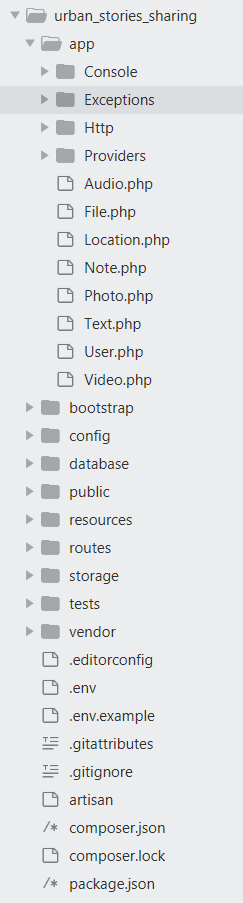
\includegraphics[width=0.2\linewidth, height=0.4\textheight]{Struttura_applicazione}
	\caption{Struttura dell'applicazione}
	\label{fig:AppStructure}
\end{figure}


La struttura dell'applicazione lato back-end, visibile in figura \ref{fig:AppStructure}, mantiene la struttura base di un'applicazione Laravel, strutturata in cartelle, ognuna delle quali contiene dei files con uno specifico compito.

\subsection{App directory}
\begin{figure}[H]
	\centering
	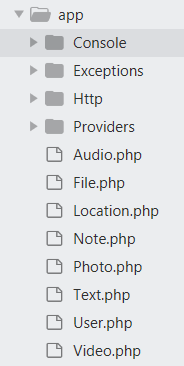
\includegraphics[width=0.15\linewidth, height=0.2\textheight]{AppDirectory}
	\caption{App directory}
	\label{fig:AppDirectory}
\end{figure}
La cartella \textit{\textbf{app}}, visibile in figura \ref{fig:AppDirectory}, contiene il codice principale dell'applicazione. Per impostazione predefinita del framework, questa directory è assegnata sotto il namespace di \textit{\textbf{App}} e viene caricata automaticamente da Composer.
Questa directory contiene tutti i modelli definiti per lo sviluppo del progetto oltre a varie sotto directory aggiuntive come Console e Http, che si possono considerare come un vero e proprio strato che fornisce un'API nel nucleo dell'applicazione.
La directory Console contiene tutti i comandi Artisan personalizzati, mentre la directory Http contiene controller e middleware, ovvero tutta logica per gestire le richieste.

\subsection{Database directory}
\begin{figure}[H]
	\centering
	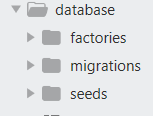
\includegraphics[width=0.2\linewidth, height=0.1\textheight]{DatabaseDirectory}
	\caption{Database directory}
	\label{fig:DBDirectory}
\end{figure}

La directory \textit{\textbf{Database}}, visibile in figura \ref{fig:DBDirectory}, contiene le migrazioni della base di dati e i file di \textit{\textbf{seeds}}, utili a popolare il modello.

\subsection{Storage directory}
La directory di archiviazione contiene l'archivio \textit{\textbf{/app/directory}} pubblico, il quale, viene utilizzato per archiviare file generati dall'utente, ovvero le note contenenti i file multimediali, che devono essere accessibili al pubblico. 
\vspace{-9px}
\section{Implementazione database}
Inizialmente, per quanto concerne la creazione del modello relazione, si era pensato di predisporre una entità autonoma per ogni tipo di file multimediale da caricare sul database, ma questo tipo di soluzione risultava ridondante poichè diverse entità presentavano gli stessi attributi, per questo motivo si è deciso di cambiare approccio e utilizzare un'entità genitore \textit{\textbf{files}}, si veda Listato \ref{lst:FilesSchema}, contenente le informazioni comuni, in relazione alle entità specializzanti per ogni tipo di file: \textit{\textbf{photos}}, \textit{\textbf{audios}} e \textit{\textbf{videos}}, visibili nel listato \ref{lst:VideosSchema}. 
\begin{lstlisting}[caption = Esempio schema tabella files, label={lst:FilesSchema}]
public function up()
{
	Schema::create('files', function (Blueprint $table) 
	{
		$table->increments('id');
		$table->float('size');
		$table->text('format');
		$table->mediumText('path')->nullable();
		$table->integer('note_id')->unsigned();
		$table->integer('photo_id')->unsigned()
			->unique()->nullable();
		$table->integer('audio_id')->unsigned()
			->unique()->nullable();
		$table->integer('video_id')->unsigned()
			->unique()->nullable();
		$table->foreign('note_id')->references('id')
			->on('notes');
		$table->foreign('photo_id')->references('id')
			->on('photos');
		$table->foreign('audio_id')->references('id')
			->on('audios');
		$table->foreign('video_id')->references('id')
			->on('videos');
		$table->timestamps();
	});
}
\end{lstlisting}
\pagebreak
\begin{lstlisting}[caption=Esempio schema tabella videos, label={lst:VideosSchema}]
public function up()
{
	Schema::create('videos', function (Blueprint $table) 
	{
		$table->increments('id');
		$table->integer('duration');
		$table->integer('width');
		$table->integer('height');
		$table->integer('bit_rate');
		$table->integer('frame_rate');
		$table->timestamps();
	});
}
\end{lstlisting}
Con lo sviluppo del progetto si è deciso di aggiungere, al modello, una nuova entità \textit{\textbf{notes}} messa in relazione con l'entità \textit{\textbf{files}}, \textit{\textbf{texts}} e \textit{\textbf{locations}}, rappresentante la geolocalizzazione delle note, che inizialmente era in relazione con l'entità \textit{\textbf{files}}.

\subsection{Codifica dei dati}
La codifica dei dati è un punto critico del progetto, poichè una scelta implementativa non ottimale potrebbe appensantire molto la base di dati.
Le due alternative possibili erano l'upload tramite \textit{\textbf{multipart form-data}} oppure tramite la \textit{\textbf{codifica in base64}}.

Dopo un'analisi delle ipotetiche dimensioni dei file salvate nel repository, si è scelto di riceve i dati codificati in \textit{\textbf{Base64}}, poiché si presuppone che le note testuali, le immagini, i file audio e i file video caricati sul server siano di piccole dimensioni.
Inoltre è stato scelto di non salvare la codifica dei dati nel database, per evitare, una volta raggiunti volumi importanti di dati, di appesantire la base di dati.
Per permettere, nonostante ciò, al client, di ricevere il file richiesto con \textit{\textbf{richieste HTTP}} di tipo \textit{\textbf{GET}}, il server si preoccupa di codificare i dati prima di essere inviati al client.

\pagebreak
\section{Implementazione web service}

Questa sezione tratta dell'implementazione del web service sviluppato per lo scambio di informazioni con la parte client, in particolare si mostrerà come vengono salvati e recuperati i file.

\subsection{Routes}

\begin{lstlisting}[caption={Definizione routes}, label={lst:RoutesDef}]
	Route::middleware('api');
	Route::get('/notes', 'NoteController@index');
	Route::get('/notes/{id}', 'NoteController@show');
	Route::get('/texts/{id}', 'TextController@show');
	Route::post('/texts', 'TextController@store');
	Route::get('/photos/{id}', 'PhotoController@show');
	Route::post('/photos', 'PhotoController@store');
	Route::get('/audios/{id}', 'AudioController@show');
	Route::post('/audios', 'AudioController@store');
	Route::get('/files/{id}', 'FileController@show');
	Route::get('/videos/{id}', 'VideoController@show');
	Route::post('/videos', 'VideoController@store');
\end{lstlisting}

Le routes, definite nel listato \ref{lst:RoutesDef}, vengono caricate dal \textit{\textbf{RouteServiceProvider}} a cui è assegnato il gruppo middleware 'api' e si occupano di instradare le richieste sui vari endpoint verso il controller dedicato.

\subsection{Controllers}

Definite le routes, sono stati realizzati i vari controller. Per ogni tipologia di file caricabile è stato definito un controller che gestisce le varie operazioni di richiesta e salvataggio dati.
Per ogni controller, quindi, sono stati definiti gli opportuni metodi che gestiscono le varie richieste HTTP;
i nomi dei metodi definiti all'interno dei controller sono stati standardizzati in modo da permettere una più semplice comprensione.

\pagebreak
\subsubsection{Metodo Index}
Il metodo \textit{\textbf{index}}, all'interno di un controller, risponde ad una richiesta di tipo \textit{\textbf{GET}} e si occupa di recuperare i file richiesti dal database. Il metodo può restituire una collezione di oggetti specifici, identificati dai parametri passati tramite query string oppure una collezione di tutte le note registrate nel database. Un esempio è riportato nel listato \ref{lst:NoteController@index}.

\begin{lstlisting}[caption={Funzione \textit{\textbf{index}} del controller NoteController},label={lst:NoteController@index}]
public function index(Request $request) {
	
	if($request->has('lat') &&
	$request->has('long')) {
	
		//Gestione dei parametri in query string
		
		return $notes;
	}
	if($request->has('type')) {

		//Gestione dei parametri in query string	
		
		return $notes;
	}
	return Note::All();
}
\end{lstlisting}

\subsubsection{Metodo Store}
Il metodo \textit{\textbf{store}} si occupa della gestione delle richieste HTTP di tipo \textit{\textbf{POST}}. 
Ovvero gestisce tutte le operazioni di salvataggio di ogni tipo di files \citep{rif2}\citep{rif4}.
Un esempio di \textit{\textbf{store}} è riportato nel listato \ref{lst:storeVideo}.

\pagebreak
\subsubsection{Metodo Show}
\begin{lstlisting}[caption={Funzione \textit{\textbf{show}} del controller NoteController}, label={lst:NoteController@show}]
public function show($id) 
{
	if(Note::find($id)){
		return Note::find($id);
	}else {
		return Response('Note not found', 404);
	}
}
\end{lstlisting}

Il un metodo \textit{\textbf{show}}, riportato nel listato \ref{lst:NoteController@show}, gestisce richieste HTTP di tipo \textit{\textbf{GET}} e ritorna un oggetto singolo che corrisponde ad un file, identificato dal parametro \textit{\textbf{id}} passato con la richiesta; il tipo dell'oggetto ritornato dipende dall'endpoint su cui si effettua la richiesta.

\subsubsection{Query string}
Quando viene effettuata una richiesta HTTP di tipo \textit{\textbf{GET}} può essere necessario passare dei parametri in \textit{\textbf{query string}} per specificare una certa tipologia di files da reperire.
Per permettere questo tipo di operazioni è stata implementata la gestione delle query string.
Sono stati previsti diversi tipi di parametri in input tramite query string. Il caso principale è quello di reperire delle note entro una certa distanza da una posizione data; per un esempio di chiamata con parametri in query string si può visionare il listato \ref{lst:QueryStringLocExample} presente in sezione \ref{sec:APIDocGetNotes}. 

La logica alla base di questa operazione, visibile nel listato \ref{lst:QueryStringLocation}, è quella di ottenere tutti i parametri passati in query string, ovvero le coordinate geografiche dell'utente e la distanza massima entro la quale si vogliono recuperare i dati; dopodichè, vengono ciclate tutte le note all'interno del repository e, sfruttando il teorema di Pitagora, vengono selezionate solo le note richieste.
\pagebreak
\begin{lstlisting}[caption={Recupero delle note entro una certa distanza da una posizione data}, label={lst:QueryStringLocation}]
foreach ($notes as $key => $value) {

	if($value->location != null) {
		$lat2 = $value->location->latitude;
		$long2 = $value->location->longitude;
		$distance = sqrt(
				pow($lat2-$lat1, 2) +
			 	pow($long2-$long1, 2)
			 	);

		if($distance > $max_distance) {
			$notes->forget($key);
		}    
	} else {
		$notes->forget($key);
	}
}
\end{lstlisting}
\pagebreak
Un altro esempio di richiesta \textit{\textbf{GET}} con parametri in query string è quello in cui si passa come parametro il tipo di file contenuto nelle note che si vuole reperire. Il codice che esegue questa operazione è riportato nel listato \ref{lst:QueryStringType}.

\begin{lstlisting}[caption={Recupero di un dato tipo di note},label={lst:QueryStringType}]
if($request->has('type')) {
	
	$request->validate([
	'type' => 'in:audio,photo,video,text'
	]);
	
	$queryStr = $request->query('type');
	$notes = collect();
	
	
	if($queryStr == 'text'){
		$texts = Text::All();
		foreach ($texts as $text) {
			$note = Note::find($text->note_id);
			$note->type = $queryStr;
			$note->content = $text->content;
			$notes->push($note);
		}
	return $notes;    
	}
	
	$files = File::whereNotNull($queryStr.'_id')->get();
	
	foreach ($files as $file) {
		$note = Note::find($file->id);
		$path = $file->path;
		$content = base64_encode(Storage::get($path));
		$note->type = $queryStr;
		$note->data = $content;
		$notes->push($note);
	}
	return $notes;
}
\end{lstlisting}

\pagebreak
\section{Archivio di salvataggio}
\begin{figure}[H]
	\centering
	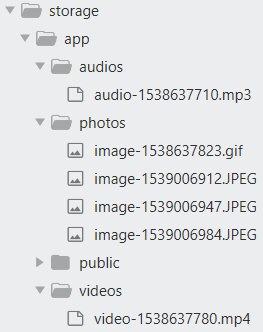
\includegraphics[width=0.3\linewidth, height=0.3\textheight]{StorageDirectory}
	\caption{Struttura directory storage}
	\label{fig:storageDirectory}
\end{figure}

L'ultima parte implementativa prevede la creazione dell'archivio in cui vengono salvati i files. Il salvataggio viene effettuato in locale e la collocazione è impostata nella directory \textit{\textbf{/storage/app/\begin{math}<\end{math}tipoFiles\begin{math}>\end{math}}} tramite i driver del disco locale.
Tutta la struttura della directory è riportata in figura \ref{fig:storageDirectory}. \\
In fase di salvataggio, dopo aver validato i parametri ricevuti in ingresso, viene generato il nome del file composto da \textit{\textbf{tipoFile-time.formatoFile}}.
Nel listato \ref{lst:storeVideo} è riportato un esempio di salvataggio di un file multimediale di tipo video.

\pagebreak
\begin{lstlisting}[caption={Esempio di salvataggio di un file video}, label={lst:storeVideo}]
public function store(Request $request)
	{
	
	//Validazione dell'input
	$validatedData = $request->validate([
		'size' => 'required|numeric',
		'format' => 'required|alpha_num',
		'duration' => 'required|numeric',
		'width' => 'required|numeric',
		'height' => 'required|numeric',
		'bit_rate' => 'required|numeric',
		'frame_rate' => 'required|numeric',
		'video_data' => 'required',
		'latitude' => 'required|numeric',
		'longitude' => 'required|numeric',
	]);
	
	//Preparazioni istanze per riempimento database record
	$video = new Video;
	$file = new File;
	$location = new Location;
	$note = new Note;
	
	//Preparazioni parametri di salvataggio
	$filename = 'video-'.time().'.'.$request['format'];
	$video_data = $request['video_data'];
	$fullPath = 'videos/'.$filename;
	
	Storage::disk('local')
		->put($fullPath, base64_decode($video_data));
	
	//Operazioni di riempimento database record
	
	return Response(['id' => $note->id], 201);
}
\end{lstlisting}


